\startchapter{Related Work}
\label{chapter:problem}

\begin{comment}
\section{Misc Notes}

\cite{Bos98} mentions that Modula-3 is used as the first year language at the State University of New York at Stony Brook, and also has a rather lengthy discussion of why Java is a poor choice as first language.

``The MIT computer science department in 1997 replaced C++ with Java as the primary software language that students were required to learn'' \cite{Benander04}  It now looks like they are moving to Python.

MIT move from Scheme to Python: http://tech.mit.edu/V125/N65/coursevi.html

\cite{Benander04} has great numbers and figures on how various institutions have moved to Java.  Also provides very strong evidence to support the claim that Java is much easier to learn if you already know OO.  Also has support for the claim that Java is easy to learn if you are already experienced as a programmer, thus possibly lend more support to the notion of ``functional first'' (though be careful, it says Java is easy to learn if you know how to program, it does not say Java is easy to learn if you know FP).

\cite{Necaise08} indicates that the popularity of python is the removal of syntax issues -- possible motivation for VPE's?
\end{comment}

\section{Practices of Teaching Introductory Programming}

\begin{flushright}
\textit{So, if I look into my foggy crystal ball at the future of computing science education, I overwhelmingly see the depressing picture of ``Business as usual''.}
\\
Edsger W. Dijkstra \cite{Dijkstra89} \\
\end{flushright}

In this section we explore how computer programming has been, currently is, and will be taught at various post-secondary institutions.  A thorough survey of the literature can be found in \cite{Pears07}.

\subsection{Curricula}

\begin{flushright}
\textit{We're not a vocational school. If someone wants to get a high-paying job, I would hope that there are easier ways to do it than working through a formal computer science curriculum.}
\\
Philip Greenspun \cite{Greenspun00} \\
\end{flushright}

Introductory programming courses should always be considered within the context of the curriculum in which they lie.  Traditionally, the introductory programming course was one of the first (or was the first) course students undertaking a degree in Computer Science would enroll, as many future Computer Science courses assume basic programming experience as a basic skill.

In North America, many introductory computing courses correspond to the guidelines outlined in the Computing Curricula recommendations by the ACM and IEEE Computer Society Joint Task Force.  The latest full curriculum recommendation came in 2001 and is known as CC2001 \cite{cc2001}.  In 2008 an interim revision from the task force was submitted \cite{cs2008}.  CC2001 identified 14 areas which comprised the body of knowledge for computer science at the undergraduate level.  These are listed in \tref{tab:CC2001BOK}.

\begin{table}
	\caption{The 14 Areas Which Comprise the CC2001 Body Of Knowledge For Computer Science}
\begin{tabular}{l}
Discrete Structures (DS) \\
Programming Fundamentals (PF) \\
Algorithms and Complexity (AL) \\
Architecture and Organization (AR) \\
Operating Systems (OS) \\
Net-Centric Computing (NC) \\
Programming Languages (PL) \\
Human-Computer Interaction (HC) \\
Graphics and Visual Computing (GV) \\
Intelligent Systems (IS) \\
Information Management (IM) \\
Social and Professional Issues (SP) \\
Software Engineering (SE) \\
Computational Science and Numerical Methods (CN) \\
\end{tabular}
	\label{tab:CC2001BOK}
\end{table}

Each of these areas are subdivided into units, and each unit consists of a number of topics.  Of the various units, some are given additional \emph{weight} in the recommendation by being designated as \emph{core} units, which are intended as being fundamental to \textbf{any} student of computer science irregardless of area of emphasis.  All units which are not designated as core units are referred to as \emph{elective} units.  While the core units comprise a fundamental set of topics for computer scientists, by themselves the core units (and the topics within) do not comprise a \emph{complete} set of material for a computer scientist -- they need to be supplemented with other elective units from other areas depending on the area of emphasis, the needs and goals of the education institution, etc.

For many years, this task force proposed a two-course introductory programming sequence commonly referred to as the CS1/CS2 sequence.  Most educational institutions in North America have followed this pattern, though the contents of the courses have evolved over time.  Roughly speaking, traditionally CS1 tends to focus on introductory programming concepts (control flow and conditional statements, variables, iteration, etc), and CS2 tends to focus more on the introduction of data structures (trees, queues, etc).  In CC2001, the importance of the object-orientated paradigm was recognized, and it was suggested that object-orientated concepts become a central part of the introductory course sequence.  Partly as a result of this addition, CC2001 also suggested a third course to follow CS2 (typically called CS3) to ensure ``students are able to master these fundamental concepts before moving on''\cite{cc2001}.  Adoption of the three course model has been mixed, with many institutions retaining the two course sequence.

\subsection{Pedagogy}

\begin{flushright}
\textit{If I could have one wish for education, it would be the systematic ordering of our basic knowledge in such a way that what is known and true can be acted on, while what is superstition, fad, and myth can be recognized as such and used only when there is nothing else to support us in our frustration and despair.}
\\
Benjamin S. Bloom \cite{Bloom72} \\
\end{flushright}

Whereas the curriculum outlines the topics that shall be introduced in a computer science curricula, an equally important (perhaps more important) aspect of the teaching of how to program is that of pedagogy.  The difference between curricula and pedagogy is well described by Pears, et al, as ``While the curriculum defines what is to be taught, pedagogy deals with the manner in which teaching and learning are managed in order to facilitate desired learning outcomes''\cite{Pears07}.  More roughly speaking, the curriculum is the ``what'' and pedagogy is the ``how''.

In the relatively short history of the discipline, there have been a number of approaches to how to introduce students to the world of computer programming.  One of the most hotly debated issues is that of the paradigm to use early on.  Traditionally, the Computing Curricula recommendations by the ACM and IEEE Computer Society Joint Task Force suggested a ``programming-first''\footnote{Sometimes this approach is referred to as ``procedural-first'', sometimes ``imperative-first''.} approach.  This style emphasized a procedural programming style early on, and many institutions still follow this model today.  However, it has been argued that this approach furthers the misconception that ``computer science equals programming'', as it puts such a heavy emphasis on programming perhaps at the expense of topics (particularly theoretical topics) more central to the discipline \cite{cc2001}.  Additionally, it has also been argued that a programming-first approach unfairly favours students with prior programming backgrounds over students with little or no background.  In addition, students who have learned some programming skills on their own before the introductory programming class tend to not have the opportunity to have poor habits corrected in the programming-first approach, as the emphasis of the approach is on simple syntactic details rather than design and algorithmic problem solving \cite{cc2001}.

As a result of many of these criticisms and potential shortcomings, as well as the increased prevalence of the paradigm, CC2001 suggested the incorporation of object-orientated principles into their introductory programming sequence.  This ``objects-first'' approach has been the source of much debate in academia since 2001 when the suggestion was made in the CC2001 guidelines, and in particular during a well documented e-mail discussion on the SIGCSE mailing list in 2004 \cite{Pausch03,Astrachan05,Hu04,Lister06}.  Some feel that the subtleties, complexities, and level of abstraction required of the object-orientated paradigm represent too great an intellectual leap for introductory programming students \cite{Hu04,Lister06}.  Some believe that the CS1/CS2 curricula is already ``too full'' as it is, without the additional complexities of the OO paradigm, and that introducing OO into the CS1/CS2 sequence will cause traditional programming constructs to be pushed by the wayside \cite{Hu04}.  Some argue that the OO paradigm is an extension of the procedural, and thus procedural programming needs to be fully understood before objects can be discussed \cite{Lister06}.  Some of the reasons for introducing objects early include the belief that since the OO paradigm is the most dominant in the world of computing, and will continue to be so for the foreseeable future, many believe that as such it is the most important for students to learn, and thus should be the first that they learn \cite{Pausch03}.  Additionally, another one of the common difficulties associated with learning the OO paradigm is that of ``paradigm shift'', and as such it has been argued that if we begin with objects early, then we avoid the paradigm shift problem \cite{Hu04,Lister06}.

In parallel to the programming-first to objects-first evolutionary approach to pedagogy, some have argued for the incorporation of functional programming into early programming courses, and propose a ``functional-first'' approach.  Much of the roots of this approach come from the text ``Structure and Interpretation of Computer Programs''\cite{SICPbook}, which was a highly influential text during the 1980's \cite{Flatt04}.  SICP, as it is commonly referred, made use of the functional programming language Scheme, and many of the exercises in the text discussed and relied on concepts from the functional paradigm (the lambda calculus, higher order functions, etc).  A well-known criticism of SICP was written by Wadler in 1987 which criticized the use of Scheme as the language, but argued in favour of retaining the functional focus of the text \cite{Wadler87}.  There has also been research done which would indicate that perhaps beginning in the object-orientated paradigm is a less desirable choice than beginning in the functional paradigm \cite{Huch05,Flatt04}.  This has significant repercussions in terms of language choice, as (for example) Java is a heavily object-orientated language, and as such it has been argued is not the ideal choice for a first year course \cite{Huch05,Bos98}.  The TeachScheme/ReachJava project shows that ``functional first'' does not imply that object-orientation must be avoided in the first year of study \cite{Bloch08,teachScheme,Felleisen04}.  Concerns with ``functional first'' include the notion that sometimes concepts that are more difficult to express in the functional paradigm are sometimes given diminished importance (I/O being the most prominent example), concerns about introducing recursion early, and the notion that functional programming is not ``mainstream'' (thus raising the ``this is not really used out in the real world'' criticism)\cite{Chakravarty04}.

In any case, all of these approaches (programming-first, objects-first, and functional-first) share a common characteristic -- they are all based upon the notion that we should structure our approach to teaching introductory programming around a particular programming paradigm.  Some however feel that this is inappropriate, that rather than focusing on a particular programming style, we should be focused on more general concepts and ideas irregardless of the paradigm.   Most notably, there has been a move toward a ``design-first'' instructional style for the introductory course.  Traditionally introductory programming courses are taught by example.  The instructor introduces a new syntactic construct from the language being used, shows a number of examples using this construct, then exercises or assignments are given where students have to take the given code from the instructor and modify it to a new problem.  Some people feel that this approach emphasizes the language more than design, and given that the specific language in use is not the primary goal of the course, it has been argued that this creates courses whereby students walk away feeling as though programming is all about learning syntax, and not about designing creative solutions to interesting problems.  The consequence of this approach is that it makes the teaching of syntax explicit and the teaching of design implicit, potentially causing courses to create students who can take existing code in Java or C++ (whichever language is used) and modify it to a new problem, but cannot design a solution to a problem from scratch.  Felleisen et al. outlines a course whereby design is made much more explicit to students, and has reported success in their approach \cite{Flatt04}.  What is interesting about this approach and others which claim to put general issues such as design as the focus, is that they are almost exclusively rooted in the functional paradigm.

\subsection{Language Choice}

\begin{flushright}
\textit{The limits of my language mean the limits of my world.}
\\
Ludwig Wittgenstein \cite{Wittgenstein22} \\
\end{flushright}

The choice of programming language for the introductory course is a critical one, though perhaps an overstated one.  Ideally the introductory programming course should be a course which teaches systematic thinking and problem solving, not ``how to write Java''.  Thus, while by necessity the introductory programming courses must make use of a programming language and environment, the primary goal of the introductory course is to teach programming in the abstract sense rather than specific syntax.

\begin{comment}
FIXME maybe drop this para:
In the history of the field, computer science has seen a variety of languages employed at one time or another as being ``the teaching language of choice''.  For our purposes we shall outline three time-frames and list some of the languages most commonly in use during those times as well as summarize findings in regards to the successes and failures of those languages from a pedagogical standpoint.
\end{comment}

In the history of the field, computer science has seen a variety of languages employed at one time or another as being ``the teaching language of choice''.  Almost as varied as the number of languages employed is the number of reasons why one language has been chosen over another.  Sometimes a language is chosen based upon faculty preference, sometimes because of industry prevalence.  Some languages are designed with learning in mind and as such have a certain appeal to educators.  Sometimes support materials in the form of programming environments or documentation will sway a department from using one language to using another.  Sometimes the paradigm chosen plays a prominent role\footnote{It would seem odd to try and teach object orientated programming in Haskell for example, as that language is based upon a different paradigm}.

Today C, C++, and Java are the most commonly used languages in both industry and education \cite{Pears07}.  Part of the appeal of these languages include the fact that they tend to be the ones most heavily used in industry.  There is additionally a sense of a movement away from C and C++ to Java as time is progressing \cite{Benander04,Bruce05}.  Various reasons have been proposed for this movement, the most common seems to be that it is a reflection of the increasing adoption of Java in industry \cite{Benander04}.  There has been considerable work done in collecting and producing resources to aid educators who are using Java in their first year courses, one of the most prominent being the ACM Java Task Force \cite{Roberts05}.

There has been considerable debate however as to whether or not Java is the most appropriate choice of language for introductory programming courses \cite{Bruce05}.  It has been shown that certain background characteristics are highly correlated with success in learning introductory programming courses for which Java is the language of choice.  The most prominent of these characteristics is prior familiarity with the object-orientated paradigm \cite{Benander04}, which is not entirely surprising given how the language is heavily based upon that paradigm.  However it is troublesome from an educational point of view in that one of the reasons Java is used in introductory programming courses is that it has been argued that it is a suitable choice for an ``objects-first'' approach due to its object-orientated nature.  Furthermore, it has been recognized that most of the programming tools which have been adopted are primarily aimed at the Java programming language.  What is not clear is whether or not this is due to a relatively widespread acceptance of the Java language, or if it is a reflection of the need for additional learning support with that language \cite{Pears07}.

Additionally there are language-specific concerns that have been raised with Java.  The ACM Java Task Force identified a Taxonomy of Problems in Teaching Java, some of which have been somewhat addressed as the language has evolved, and some of which remain problems to this day \cite{acmJavaForce04}.  The difficulties are summarized in \tref{tab:ACMJTFPROB}.

\begin{table}
	\caption{Summary of Problems in Teaching Java\cite{acmJavaForce04}}
\begin{tabular}{c p{3in} r}
\hline
\multicolumn{3}{l}{\emph{High Level Issues}} \\
H1 & Scale & (remains a concern) \\
H2 & Instability & (remains a concern) \\
H3 & Speed of Execution & (improving over time) \\
H4 & Lack of good textbooks and environments & (improving over time) \\
\hline
\multicolumn{3}{l}{\emph{Language Issues}} \\
L1 & Static methods, including \code{main} & (remains a concern) \\
L2 & Exceptions & (remains a concern) \\
L3 & Poor separation of interface and implementation & (partly addressed by tools) \\
L4 & Wrapper classes & (added in Java 5.0) \\
L5 & Lack of parameterized types & (added in Java 5.0) \\
L6 & Lack of enumerated types & (added in Java 5.0) \\
L7 & Inability to code preconditions & (added in JDK 1.4) \\
L8 & Lack of an iterator syntax & (added in Java 5.0) \\
L9 & Low-level concerns & (disposition varies) \\
\hline
\multicolumn{3}{l}{\emph{API Issues}} \\
A1 & Lack of a simple input mechanism & (remains a concern) \\
A2 & Conceptual difficulty of the graphics model & (remains a concern) \\
A3 & GUI Components inappropriate for beginners & (remains a concern) \\
A4 & Inadequate support for event-driven code & (remains a concern) \\
\hline
\end{tabular}
	\label{tab:ACMJTFPROB}
\end{table}

As the result of the difficulties associated with the use of C/C++ and Java in the introductory programming course, many institutions are now switching from C/C++ and/or Java to other languages.  The most common of these is the Python programming language \cite{python}.  Python has the advantage of being a scripted, interpreted language, thus students can ``try-out'' small expressions or snippets of code without having to get a complete source file free from errors.  It also has a relatively ``clean'' and simple syntax compared to the relatively verbose Java.  The use of whitespace for program structure encourages good indentation habits early as well.  With all these benefits it is not surprising to see some institutions beginning to adopt Python as the language for their introductory programming courses.  Perhaps the most notable adoption of Python happened at MIT, whose Computer Science department had long been a strong proponent of the use of Scheme in introductory programming courses due to the adoption of \cite{SICPbook} as the introductory text \cite{Thetech06}.  Other examples of using Python in CS1/CS2 style courses and the possible benefits and drawbacks of doing so can be found in \cite{Radenski06,Shannon03,Agarwal05,Agarwal08}.  While there have been successes with Python in the classroom, not even the strongest supporters of the language claim that it is the ``perfect choice''.

\section{Visual Programming Environments}
\label{sec:vpes}

\begin{flushright}
\textit{Like Moses, I get to see the promised land, but not set foot in it.  \\
But the vision is clear.}
\\
Randy Pausch \cite{Pausch08} \\
\end{flushright}

One of the major difficulties associated with learning to program is the issue of syntax errors, and as a result of this, there has been a great deal of work done attempting to minimize or reduce this hurdle \cite{Kelleher05}.  One of the major categories of this work is the world of the visual programming environment (VPE)\footnote{Some authors use the term ``visual programming language'' rather than ``visual programming environment''}.  A VPE is a programming environment where the user interacts with graphical on-screen objects rather than the traditional textual method of writing text-based code.  Another definition comes from Kelleher \& Pausch:

\begin{quotation}
...[VPE's] use graphical or physical objects to represent elements of a program such as commands, control structures, or variables. These objects can be moved around and combined in different ways to form programs. Novice programmers need only to recognize the names of commands and the syntax of the statements is encoded in the shapes of the objects, preventing them from creating syntactically incorrect statements \cite{Kelleher05}.
\end{quotation}

\subsection{Criticisms of Visual Programming Environments}

There are two common criticisms of VPE's that have somewhat slowed their adoption: the scaling-up problem, and concerns about transfer of training.  The scaling-up problem refers to the programmer's ability to apply VPE's in larger programs.  That is, questions have been raised about whether or not the visual representation used in VPE's ultimately are too unwieldy to produce programs of moderate complexity \cite{Burnett94}.  Transfer of training concerns whether or not skills and knowledge acquired in a VPE can be transferred to a traditional text-based environment in the future.  Some support for the claim that a visual environment can provide positive ``transfer of training'' to a textual environment can be found in \cite{Hundhausen09}.

\subsection{Examples of Visual Programming Environments}

There have been a number of VPE's proposed, we shall focus on a few environments which have proven to be of great influence particularly in regards to the educational side of Computer Science.  A more thorough discussion of other VPE's can be found in \cite{Kelso02} and \cite{Kelleher05}.

An early VPE system that has proven to be quite influential is Prograph, a visual object-orientated dataflow language.  Objects in Prograph are modeled as on-screen hexagons, with one half of the hexagon representing the data attributes of the object, and the other half the methods.  By double-clicking on a part of the object a user can explore further the various methods and attributes of the object.  Methods are contained in ``frames'', which are represented as directed graphs.  Nodes in the graph are icons representing various constructs (objects, methods, conditionals, etc) and are connected together.  Flow of data proceeds from the top of the digraph, passing through the various instructions, down to the bottom of the digraph, and outward (if the method has output).  One of the major influences of Prograph was this ``box and wire'' representation, as it was one of the earlier systems to make use of it, and many VPE's have also made use of this metaphor.  As well, Prograph has become something of a benchmark system in evaluating VPE's\footnote{Green uses Prograph and LabVIEW as the two model systems which he applies his Cognitive Dimensions Framework to}.  It would appear however, that active development on Prograph ceased in the early 1990's.

Another VPE that is somewhat similar to Prograph is LabVIEW\cite{labview}, a visual environment used for designing electronic circuits.  That is, it uses ``the metaphor of an electric circuit as a programming model''\cite{Kelso02}.  It also has a dataflow-style, whereby components are connected together, and data ``flows'' through the network of components.  It also, like Prograph, makes use of the ``box-and-wire'' representation.  It is a proprietary product of the National Instruments corporation, and also has been used as a ``model'' language when evaluating VPE's.

Neither of the above two environments are based upon the functional paradigm however.  One such environment that is heavily based upon the functional paradigm is the VFPE\footnote{Short for ``Visual Functional Programming Environment''}, developed by Kelso \cite{Kelso02}.  The VFPE shares a common computational model with existing functional languages (such as Haskell).  One of the central points of Kelso's work is the argument that functional languages have a unique singular visual representation -- the syntax tree.  As such, the VFPE is in many ways just a visual representation of that tree.  A screenshot of the VFPE can be seen in \fref{fig:vfpe}.  The main interface to the VFPE consists of a main expression window (seen in \fref{fig:vfpe-main}) which contains the program being constructed.  Components are selected from the menus on the right half of this interface, and dropped into placeholders in the main expression.  Functions can be defined, and the definition of sub functions are done in a separate window called a binding frame (as seen in \fref{fig:vfpe-sub}).  Note that the layout of components is done by the environment, it is not ``freeform'' as users cannot control where components are laid out in the main expression window.

\begin{figure}[htp]
  \begin{center}
    \subfloat[The Main VFPE Window]{\label{fig:vfpe-main}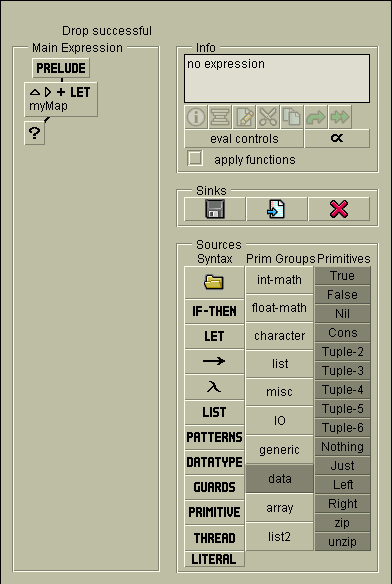
\includegraphics[scale=0.4]{Figures/vfpeMain}} \quad
    \subfloat[A Binding Frame in VFPE]{\label{fig:vfpe-sub}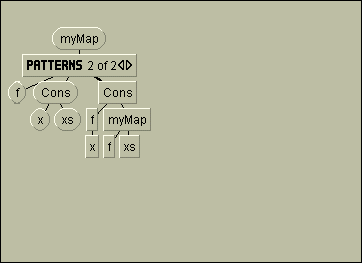
\includegraphics[scale=0.4]{Figures/vfpeSub}}
  \end{center}
  \caption{The Visual Functional Programming Environment (VFPE)}
  \label{fig:vfpe}
\end{figure}

\begin{comment}
Alice, Scratch, Gamemaker, VFPE, Prograph

Use of Game Maker in educational setting at UVic can be found in \cite{Gooch08}.
\end{comment}

\section{Games and Computer Science Curricula}
\label{chapter:problemSec:games}

\begin{flushright}
\textit{College students today have been called the ``Nintendo generation'' or the ``MTV generation.'' Their perception of technology and media has been profoundly influenced by these sources. ...these are the kinds of media that Nintendo generation students want to produce when learning computer science.}
\\
Mark Guzdial and Elliot Soloway \cite{Guzdial02} \\
\end{flushright}

In recent years there has been a notable decline in enrollment in Computer Science courses \cite{Manaris07,Vesgo07,Ward08,Bayliss09}.  As a result of this decline, many institutions are seeking out interesting and new ways to ``entice'' students to enroll in Computer Science courses and to rekindle interest in the discipline.  One such method that has been proposed is to incorporate computer games into Computer Science curricula.  Cliburn et al. provides a summary of how games have been used in this fashion in \cite{Cliburn06}.

The rationale behind this move is that since video games are an exciting and compelling application of computer programming, that perhaps that interest in games can be leveraged by instructors in their introductory programming courses and beyond \cite{Barnes08,Sweedyk05,Overmars04}.  Furthermore, video games are a multi-billion dollar industry \cite{Wallace06}, and a common motivation for students in choosing a discipline are the employment opportunities a degree in the field would entail.  Since electronic entertainment is so prosperous, having curricula that targets students specifically for this field can be a compelling factor in one choosing a degree in Computer Science.

Some institutions have even taken this move a step further and are now offering gaming themes and concentrations in their degrees.  Recently, the University of Victoria added a ``Graphics and Gaming'' option to their Computer Science major program.  Other attempts at this are explored in \cite{Leutenegger07,Murray06,Zyda06}.  Most institutions that incorporate games into their courses or degrees have reported an increase in student enjoyment.  It has been shown that students prefer assignments based around games than ``traditional'' or ``story-telling'' assignments \cite{Cliburn08}.

%\cite{Cliburn08} provides strong evidence that in a general, aggregate study, students prefer assignments based around games than ``traditional'' or ``story-telling'' assignments.

While there have been successes reported surrounding the use of games, it is very much a controversial choice, as there are a number of concerns that have been raised in regards to gaming-centered curricula.  There is strong evidence to indicate that while gaming may spark initial interest in computing, it does not follow that this initial interest will translate into increases in students undertaking Computer Science majors.  A survey of 1,872 students conducted at a ``highly selective public technical university'' found that while 43\% of students indicated that games influenced their interest in computing, only 6.9\% realized that interest by becoming Computer Scientists \cite{DiSalvo09}.  Furthermore, while student interest generally seems to increase with assignments making use of games, few institutions have reported any noticible improvement in student performance.  Cliburn reported findings of a study he performed in the introductory programming course at Hanover College and found that students had a higher overall average score (95.1\% on average) on traditional assignments than on game-based assignments (89.1\% on average)\cite{Cliburn06}.  Interestingly, he also found that in spite of this, most students (78.9\%) still preferred game-based assignments over ``traditional'' assignments, perhaps a further testament to the motivating power of games as assignments.

Concerns have also been raised surrounding issues of gender and race.  One such concern suggests that games appeal more to male students than female, and that incorporation of games may alienate females from the discipline.  Specifically, there has been evidence to show that females tend to prefer games which are cooperative in nature rather than competitive, and that the latter can deter interest of women in games \cite{Camp02}.  This would indicate that educators must be careful about how they incorporate games into courses, and to design course materials with this concern in mind \cite{Carmichael08}.  Other works have adopted ``story-telling'' rather than games as being the vehicle of motivation, and have specifically explored this avenue with middle-school girls with great success \cite{Kelleher06}.

\begin{comment}
\cite{Natvig04,Barnes08} example of games being used
Some ideas about why creativity is important can be found in \cite{Farooq06}.
Games as a motivational tool: see ``International Conference on Game Development in Computer Science Education''.
An excellent outline of how games can be used successfully in CS curricula as well as how not only should we shoehorn games but also focus on fundamentals is summarized in \cite{Bayliss09}.  It also discusses what considerations should be made when incorporating games into courses.
\end{comment}

